\documentclass[10pt,a4paper]{article}

\usepackage[margin=0.75cm]{geometry}
\usepackage[utf8]{inputenc}

\usepackage{amsmath}
\usepackage{amssymb}
\usepackage[backend=biber]{biblatex}
\usepackage{textcomp}
\usepackage{gensymb}
\usepackage{paracol}
\usepackage{parskip}
\usepackage{tikz}
\usepackage{titlesec}
\usepackage{verbatim}
\usepackage{xcolor}

\titleformat{\section}[block]{\Large\bfseries\filcenter\color{red}}{\thesection}{1em}{}[\hrule]
\titleformat{\subsection}[block]{\bfseries\filcenter\color{red}}{\thesubsection}{1em}{}[\hrule]

\setlength{\columnsep}{25pt}

\begin{comment}
    Algebra (Linear and Groups) = red
    Calculus = cyan
    Complex Variables = violet
    Differential Equations = blue
    Discrete Mathematics (incl. Algorithms, Data Structures and Graphs) = teal
    Probability & Statistics = orange
    Physics = purple
    Chemistry = olive
    Biology = magenta

    Artificial Intelligence = pink
    Cognitive Science = purple
    Machine Learning = cyan
    Probabilistic Modelling and Reasoning = orange
    Neural Networks = blue
    Information Retrieval and Search Engines = olive
    Bioinformatics = magenta
    Reinforcement Learning = teal
    SVMs = red
    Knowledge Representation = violet
\end{comment}

\tikzset{
    rounded-box/.style = {draw=red, fill=white, thin, rectangle, rounded corners, inner sep=5pt, inner ysep=10pt},
    rounded-box-title/.style = {fill=red, text=white, font=\bfseries},
}

\addbibresource{references.bib}

\begin{document}
\title{Cheat Sheet}

\input{section-1-vectors}
\input{section-2-systems-of-linear-equations}
\input{section-3-linear-independence} \newpage
\input{section-4-linear-subspaces}
\input{section-5-orthogonality} \newpage
\input{section-6-least-squares}
\input{section-7-matrix-algebra} \newpage
\input{section-8-linear-transformations} \newpage
\input{section-9-determinants} \newpage
\input{section-10-eigenvalues-and-eigenvectors}
\input{section-11-similarity-and-diagonalisation} \newpage
\input{section-12-symmetric matrices} \newpage
\input{section-13-vector-spaces} \newpage
\section{Relations}

\begin{paracol}{2}

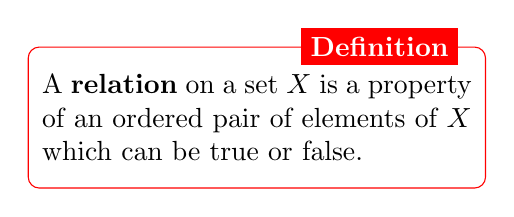
\begin{tikzpicture}
\node [rounded-box] (box){\begin{minipage}{0.45\textwidth}
    A \textbf{relation} on a set $X$ is a property of an ordered pair of elements of $X$ which can be true or false.
\end{minipage}};
\node[rounded-box-title, left=10pt] at (box.north east) {Definition};
\end{tikzpicture}

\textbf{Example}: $<$ is a relation on the set of natural numbers: if $a$ and $b$ are natural numbers then $a < b$ is either true or false.

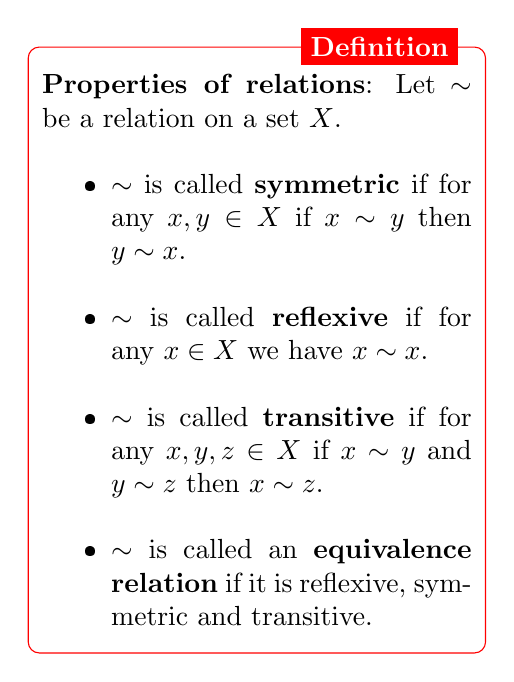
\begin{tikzpicture}
\node [rounded-box] (box){\begin{minipage}{0.45\textwidth}
    \textbf{Properties of relations}: Let $\sim$ be a relation on a set $X$. \\

    \begin{itemize}
        \item $\sim$ is called \textbf{symmetric} if for any $x, y \in X$ if $x \sim y$ then $y \sim x$. \\

        \item $\sim$ is called \textbf{reflexive} if for any $x \in X$ we have $x \sim x$. \\

        \item $\sim$ is called \textbf{transitive} if for any $x, y, z \in X$ if $x \sim y$ and $y \sim z$ then $x \sim z$. \\

        \item $\sim$ is called an \textbf{equivalence relation} if it is reflexive, symmetric and transitive.
    \end{itemize}
\end{minipage}};
\node[rounded-box-title, left=10pt] at (box.north east) {Definition};
\end{tikzpicture}

\switchcolumn

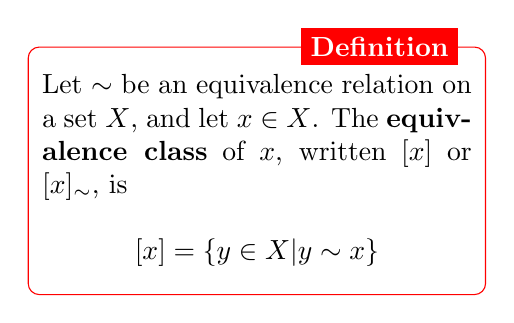
\begin{tikzpicture}
\node [rounded-box] (box){\begin{minipage}{0.45\textwidth}
    Let $\sim$ be an equivalence relation on a set $X$, and let $x \in X$. The \textbf{equivalence class} of $x$, written $[x]$ or $[x]_\sim$, is

    $$[x] = \{ y \in X | y \sim x \}$$
\end{minipage}};
\node[rounded-box-title, left=10pt] at (box.north east) {Definition};
\end{tikzpicture}

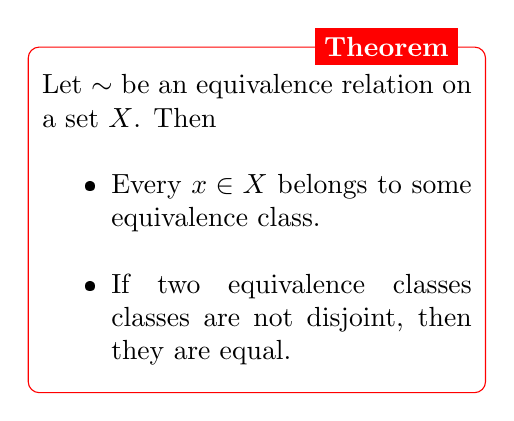
\begin{tikzpicture}
\node [rounded-box] (box){\begin{minipage}{0.45\textwidth}
    Let $\sim$ be an equivalence relation on a set $X$. Then \\

    \begin{itemize}
        \item Every $x \in X$ belongs to some equivalence class. \\

        \item If two equivalence classes classes are not disjoint, then they are equal.
    \end{itemize}
\end{minipage}};
\node[rounded-box-title, left=10pt] at (box.north east) {Theorem};
\end{tikzpicture}

\end{paracol}

\section{Functions}

\begin{paracol}{2}

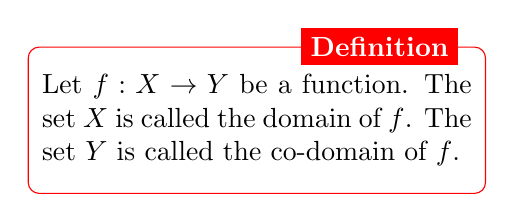
\begin{tikzpicture}
\node [rounded-box] (box){\begin{minipage}{0.45\textwidth}
    Let $f: X \rightarrow Y$ be a function. The set $X$ is called the domain of $f$. The set $Y$ is called the co-domain of $f$.
\end{minipage}};
\node[rounded-box-title, left=10pt] at (box.north east) {Definition};
\end{tikzpicture}

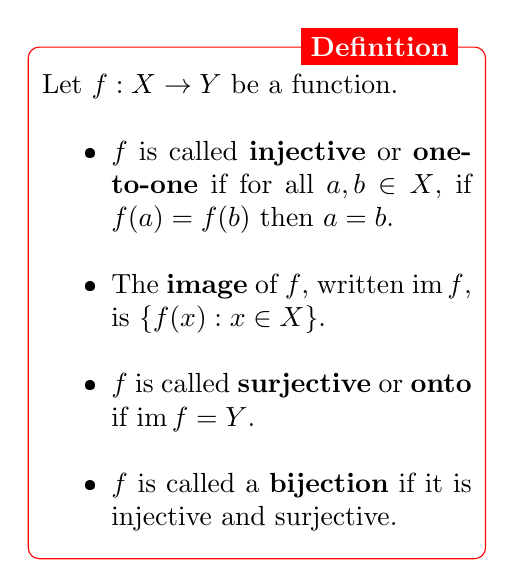
\begin{tikzpicture}
\node [rounded-box] (box){\begin{minipage}{0.45\textwidth}
    Let $f: X \rightarrow Y$ be a function. \\

    \begin{itemize}
        \item $f$ is called \textbf{injective} or \textbf{one-to-one} if for all $a, b \in X$, if $f(a) = f(b)$ then $a = b$. \\

        \item The \textbf{image} of $f$, written $\text{im} \, f$, is $\{ f(x) : x \in X \}$. \\

        \item $f$ is called \textbf{surjective} or \textbf{onto} if $\text{im} \, f = Y$. \\

        \item $f$ is called a \textbf{bijection} if it is injective and surjective.
    \end{itemize}
\end{minipage}};
\node[rounded-box-title, left=10pt] at (box.north east) {Definition};
\end{tikzpicture}

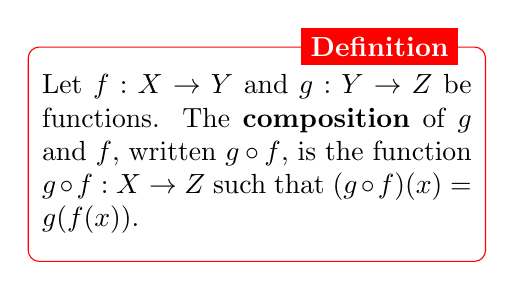
\begin{tikzpicture}
\node [rounded-box] (box){\begin{minipage}{0.45\textwidth}
    Let $f: X \rightarrow Y$ and $g: Y \rightarrow Z$ be functions. The \textbf{composition} of $g$ and $f$, written $g \circ f$, is the function $g \circ f : X \rightarrow Z$ such that $(g \circ f)(x) = g(f(x))$.
\end{minipage}};
\node[rounded-box-title, left=10pt] at (box.north east) {Definition};
\end{tikzpicture}

NB: Composition only makes sense when the co-domain of $f$ is the same as the domain of $g$.

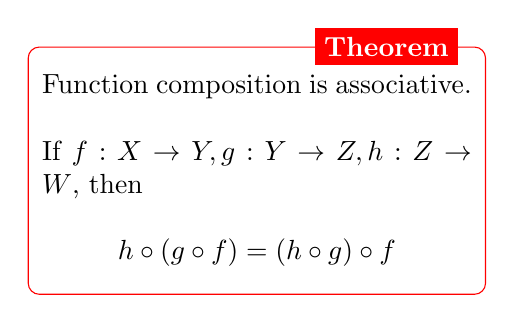
\begin{tikzpicture}
\node [rounded-box] (box){\begin{minipage}{0.45\textwidth}
    Function composition is associative. \\

    If $f: X \rightarrow Y, g: Y \rightarrow Z, h: Z \rightarrow W$, then

    $$h \circ (g \circ f) = (h \circ g) \circ f$$
\end{minipage}};
\node[rounded-box-title, left=10pt] at (box.north east) {Theorem};
\end{tikzpicture}

The reason this is true is because both sides send an input $x \in X$ to the output $h(g(f(x)))$.

\switchcolumn

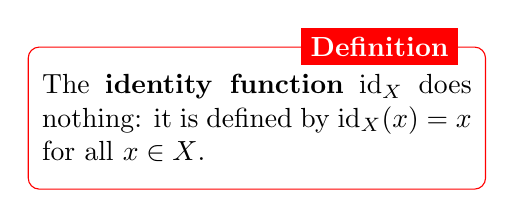
\begin{tikzpicture}
\node [rounded-box] (box){\begin{minipage}{0.45\textwidth}
    The \textbf{identity function} $\text{id}_X$ does nothing: it is defined by $\text{id}_X(x) = x$ for all $x \in X$.
\end{minipage}};
\node[rounded-box-title, left=10pt] at (box.north east) {Definition};
\end{tikzpicture}

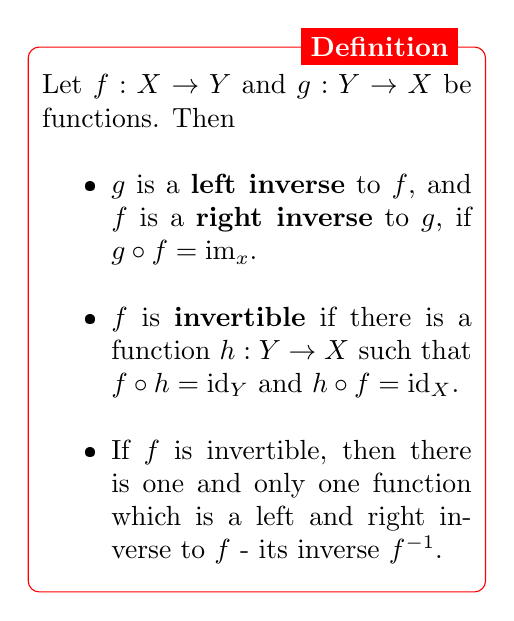
\begin{tikzpicture}
\node [rounded-box] (box){\begin{minipage}{0.45\textwidth}
    Let $f: X \rightarrow Y$ and $g: Y \rightarrow X$ be functions. Then \\

    \begin{itemize}
        \item $g$ is a \textbf{left inverse} to $f$, and $f$ is a \textbf{right inverse} to $g$, if $g \circ f = \text{im}_x$. \\

        \item $f$ is \textbf{invertible} if there is a function $h: Y \rightarrow X$ such that $f \circ h = \text{id}_Y$ and $h \circ f = \text{id}_X$. \\

        \item If $f$ is invertible, then there is one and only one function which is a left and right inverse to $f$ - its inverse $f^{-1}$.
    \end{itemize}
\end{minipage}};
\node[rounded-box-title, left=10pt] at (box.north east) {Definition};
\end{tikzpicture}

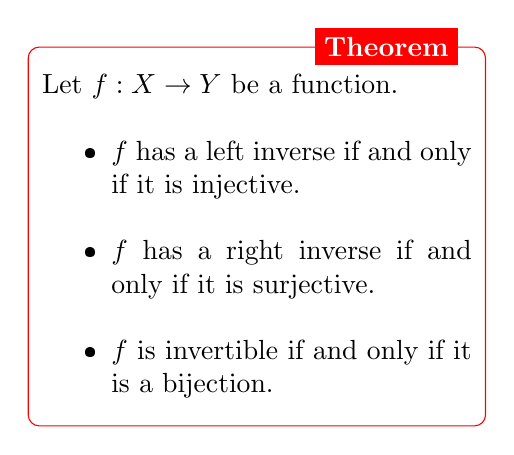
\begin{tikzpicture}
\node [rounded-box] (box){\begin{minipage}{0.45\textwidth}
    Let $f: X \rightarrow Y$ be a function. \\

    \begin{itemize}
        \item $f$ has a left inverse if and only if it is injective. \\

        \item $f$ has a right inverse if and only if it is surjective. \\

        \item $f$ is invertible if and only if it is a bijection.
    \end{itemize}
\end{minipage}};
\node[rounded-box-title, left=10pt] at (box.north east) {Theorem};
\end{tikzpicture}

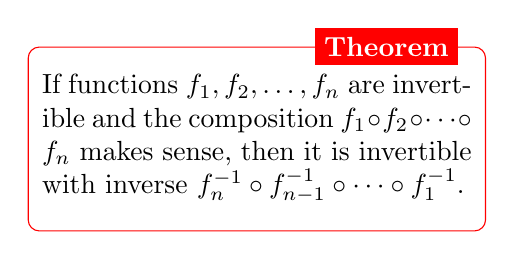
\begin{tikzpicture}
\node [rounded-box] (box){\begin{minipage}{0.45\textwidth}
    If functions $f_1, f_2, \dots, f_n$ are invertible and the composition $f_1 \circ f_2 \circ \dots \circ f_n$ makes sense, then it is invertible with inverse $f_n^{-1} \circ f_{n-1}^{-1} \circ \dots \circ f_1^{-1}$.
\end{minipage}};
\node[rounded-box-title, left=10pt] at (box.north east) {Theorem};
\end{tikzpicture}

\end{paracol}

\section{Permutations}

\begin{paracol}{2}

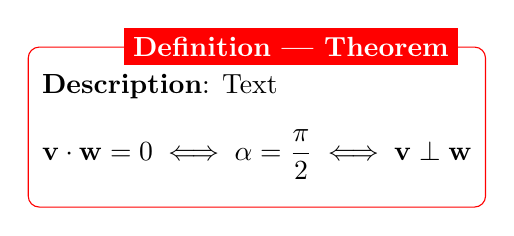
\begin{tikzpicture}
\node [rounded-box] (box){\begin{minipage}{0.45\textwidth}
    \textbf{Description}: Text
    $$\mathbf{v} \cdot \mathbf{w} = 0 \iff \alpha = \frac{\pi}{2} \iff \mathbf{v} \perp \mathbf{w}$$
\end{minipage}};
\node[rounded-box-title, left=10pt] at (box.north east) {Definition | Theorem};
\end{tikzpicture}

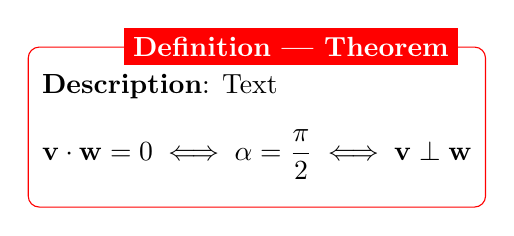
\begin{tikzpicture}
\node [rounded-box] (box){\begin{minipage}{0.45\textwidth}
    \textbf{Description}: Text
    $$\mathbf{v} \cdot \mathbf{w} = 0 \iff \alpha = \frac{\pi}{2} \iff \mathbf{v} \perp \mathbf{w}$$
\end{minipage}};
\node[rounded-box-title, left=10pt] at (box.north east) {Definition | Theorem};
\end{tikzpicture}

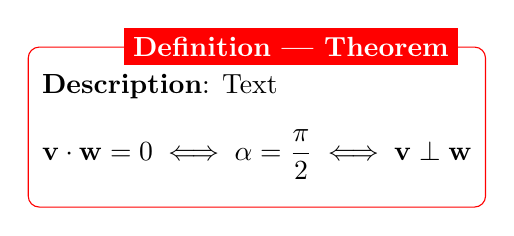
\begin{tikzpicture}
\node [rounded-box] (box){\begin{minipage}{0.45\textwidth}
    \textbf{Description}: Text
    $$\mathbf{v} \cdot \mathbf{w} = 0 \iff \alpha = \frac{\pi}{2} \iff \mathbf{v} \perp \mathbf{w}$$
\end{minipage}};
\node[rounded-box-title, left=10pt] at (box.north east) {Definition | Theorem};
\end{tikzpicture}

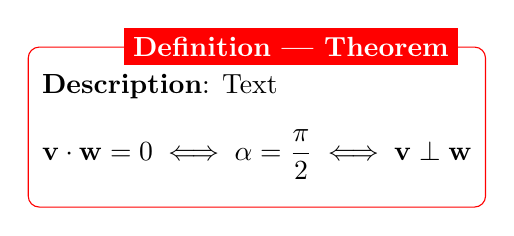
\begin{tikzpicture}
\node [rounded-box] (box){\begin{minipage}{0.45\textwidth}
    \textbf{Description}: Text
    $$\mathbf{v} \cdot \mathbf{w} = 0 \iff \alpha = \frac{\pi}{2} \iff \mathbf{v} \perp \mathbf{w}$$
\end{minipage}};
\node[rounded-box-title, left=10pt] at (box.north east) {Definition | Theorem};
\end{tikzpicture}

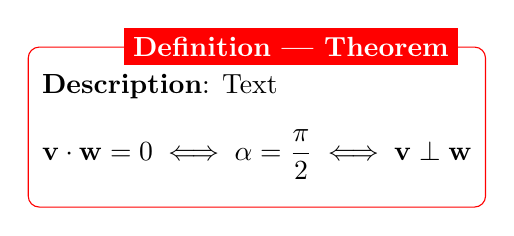
\begin{tikzpicture}
\node [rounded-box] (box){\begin{minipage}{0.45\textwidth}
    \textbf{Description}: Text
    $$\mathbf{v} \cdot \mathbf{w} = 0 \iff \alpha = \frac{\pi}{2} \iff \mathbf{v} \perp \mathbf{w}$$
\end{minipage}};
\node[rounded-box-title, left=10pt] at (box.north east) {Definition | Theorem};
\end{tikzpicture}

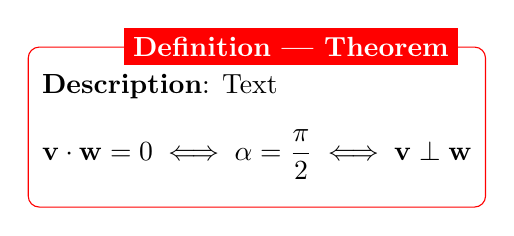
\begin{tikzpicture}
\node [rounded-box] (box){\begin{minipage}{0.45\textwidth}
    \textbf{Description}: Text
    $$\mathbf{v} \cdot \mathbf{w} = 0 \iff \alpha = \frac{\pi}{2} \iff \mathbf{v} \perp \mathbf{w}$$
\end{minipage}};
\node[rounded-box-title, left=10pt] at (box.north east) {Definition | Theorem};
\end{tikzpicture}

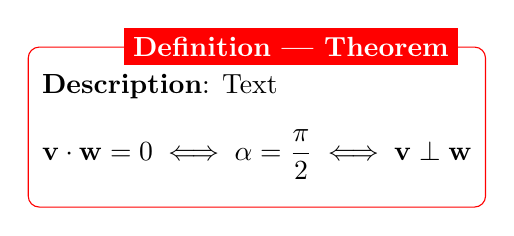
\begin{tikzpicture}
\node [rounded-box] (box){\begin{minipage}{0.45\textwidth}
    \textbf{Description}: Text
    $$\mathbf{v} \cdot \mathbf{w} = 0 \iff \alpha = \frac{\pi}{2} \iff \mathbf{v} \perp \mathbf{w}$$
\end{minipage}};
\node[rounded-box-title, left=10pt] at (box.north east) {Definition | Theorem};
\end{tikzpicture}

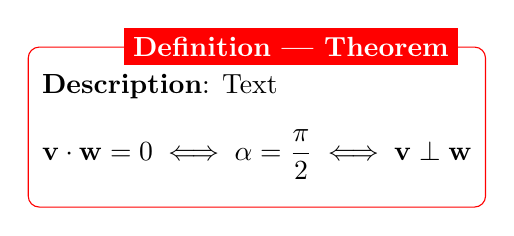
\begin{tikzpicture}
\node [rounded-box] (box){\begin{minipage}{0.45\textwidth}
    \textbf{Description}: Text
    $$\mathbf{v} \cdot \mathbf{w} = 0 \iff \alpha = \frac{\pi}{2} \iff \mathbf{v} \perp \mathbf{w}$$
\end{minipage}};
\node[rounded-box-title, left=10pt] at (box.north east) {Definition | Theorem};
\end{tikzpicture}

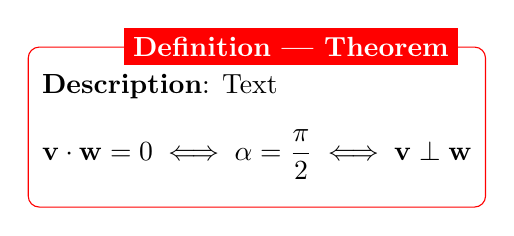
\begin{tikzpicture}
\node [rounded-box] (box){\begin{minipage}{0.45\textwidth}
    \textbf{Description}: Text
    $$\mathbf{v} \cdot \mathbf{w} = 0 \iff \alpha = \frac{\pi}{2} \iff \mathbf{v} \perp \mathbf{w}$$
\end{minipage}};
\node[rounded-box-title, left=10pt] at (box.north east) {Definition | Theorem};
\end{tikzpicture}

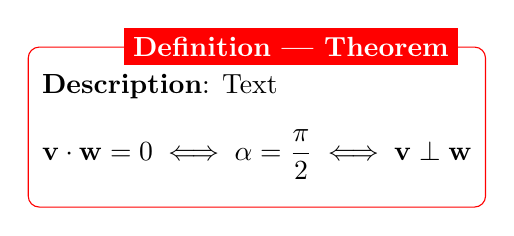
\begin{tikzpicture}
\node [rounded-box] (box){\begin{minipage}{0.45\textwidth}
    \textbf{Description}: Text
    $$\mathbf{v} \cdot \mathbf{w} = 0 \iff \alpha = \frac{\pi}{2} \iff \mathbf{v} \perp \mathbf{w}$$
\end{minipage}};
\node[rounded-box-title, left=10pt] at (box.north east) {Definition | Theorem};
\end{tikzpicture}

\end{paracol}
 \newpage
\input{section-15-groups} \newpage
\input{section-16-the-symmetric-group} \newpage
\input{section-17-subgroups} \newpage
\input{section-18-cosets-and-lagranges-theorem} \newpage
\input{section-19-the-dihedral-groups} \newpage
\section{Homomorphisms and Isomorphisms}

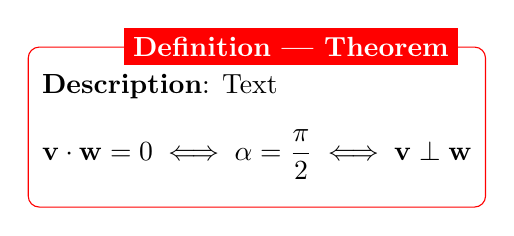
\begin{tikzpicture}
\node [rounded-box] (box){\begin{minipage}{0.45\textwidth}
    \textbf{Description}: Text
    $$\mathbf{v} \cdot \mathbf{w} = 0 \iff \alpha = \frac{\pi}{2} \iff \mathbf{v} \perp \mathbf{w}$$
\end{minipage}};
\node[rounded-box-title, left=10pt] at (box.north east) {Definition | Theorem};
\end{tikzpicture}
 \newpage

\nocite{*}
\printbibliography

\end{document}
